%\documentclass[draft]{agujournal2018}
\documentclass[]{agujournal2018}
\usepackage{apacite}
\usepackage{url}
\usepackage{lineno}
%\linenumbers
\draftfalse
\journalname{Geophysical Research Letters}

%custom packages
\usepackage{amsmath,amssymb,amsfonts,amsthm}
\usepackage{comment}
\usepackage{booktabs}
% custom commands
\newcommand\be{\begin{equation}}
\newcommand\ee{\end{equation}} 
\newcommand\bra{\langle}
\newcommand\ket{\rangle}
\newcommand\om{\omega}
\newcommand\tom{\tilde{\omega}}
\newcommand\tg{\tilde{g}}
\newcommand\tp{\tilde{p}}
\newcommand\tG{\tilde{G}}
\newcommand\El{\mathcal{L}}
%\usepackage{layouts}
%\printinunitsof{in}\prntlen{\textwidth} % check scales in the document


\begin{document}

\title{Back to Einstein: how to include burial in fluvial sediment diffusion models?}

\authors{James K. Pierce \affil{1}and Marwan A. Hassan\affil{1}}
\affiliation{1}{Department of Geography \\University of British Columbia}
\correspondingauthor{James Kevin Pierce}{kpierce@alumni.ubc.ca}

\begin{keypoints}
\item We develop a random-walk model of objects in intermittent transport through an environment with traps
\item Its solution provides three ranges of diffusion, two of which are anomalous
\item We apply the model to sediment transport in rivers to clarify the scale-dependence of bedload diffusion

\end{keypoints}

\begin{abstract}
Sediment grains transport through gravel-bed rivers in cycles of motion and rest.
When grains rest on the surface, material transported from upstream can bury them.
Grains on the surface shield buried grains from the flow, so they can be immobile for long time periods.
These immobile periods can dominate sediment diffusion characteristics. 
Despite the significant impact of sediment burial on diffusion, nearly all existing models neglect it.
In this letter, we present a random walk model incorporating sediment burial and solve it analytically.
The model predicts three sediment diffusion ranges with distinct scaling characteristics in each.
We relate the crossover times dividing these ranges to measurable transport parameters and describe each range from underlying physical processes.
Our developments provide new geophysical perspective on the scale-dependence of fluvial sediment transport.
\end{abstract}

\section{Introduction}

Anomalous diffusion has attracted considerable research attention in recent times, emerging in diverse contexts including the transport of cholesterols through lipid bilayers \citep{Jeon2012,Molina-Garcia2018}, contaminants through soils \citep{Berkowitz2006,Yang2019}, and pollinator insects through ecosystems \citep{Reynolds2009,Vallaeys2017}.
In this letter, we study anomalous diffusion in a river science context, where it emerges from the transport of coarse bedload sediment through river channels \citep{Bradley2017,Martin2012}.
\citet{Einstein1937} developed the first model of bedload diffusion to describe his comprehensive experiments tracing painted grains through a flume in Meyer-Peter's laboratory \citep{Ettema2004}.
Diffusion is the spreading apart of grains as they transport downstream, and it is induced by differences in the transport characteristics of one grain and the next. Diffusion is usually quantified by the time dependence of the positional variance $\sigma_x^2(t)$ of a population.
When $\sigma_x^2 \propto t$, the diffusion is said to be normal, since this is found in the classic diffusion problems \citep[e.g.][]{Einstein1905,Taylor1920}.
However, many transport phenomena show $\sigma_x^2 \propto t^\gamma$ with $\gamma \neq 1$. This diffusion is said to be anomalous \citep{Sokolov2012}. If $\gamma>1$, it is said to be super-diffusive; while if $\gamma <1$, it is said to be sub-diffusive \citep{Metzler2000}.
Einstein concluded from his experiments and modeling that bedload transport expresses normal diffusion.

Researchers after Einstein have come to recognize that coarse sediment moving through river channels can show either anomalous or normal diffusion depending on the timescale of observation \citep{Nikora2002}.
This is a significant issue since it implies diffusion models should be scale dependent, and it renders experimental data contingent on their observation timescales.
\citet{Nikora2001a,Nikora2002} were the first to fundamentally rework Einstein's concept of bedload diffusion.
They identified three ranges of diffusion from Newtonian simulations and experimental data, and they termed these ranges local, intermediate, and global in order of increasing timescale.
They determined that $\sigma_x^2$ scales with a different power of time in each range, and they concluded this scaling could be either anomalous or normal.
More recent works have more or less supported the Nikora et al. findings.
Various numerical approaches show two \citep[e.g.][]{Fan2016} or three \citep[e.g.][]{Bialik2012,Zhang2012} ranges of diffusion; one set of flume experiments appears to show two ranges of sediment diffusion \citep{Martin2012}, and several field studies have shown anomalous diffusion \citep{Bradley2017, Phillips2013}
However, the full picture of scale-dependent bedload diffusion is far from clear.
In particular, we are not able to (super/normal/subdiffusion) of each range (local/intermediate/global), and no model has been developed, to our knowledge, that derives all three diffusion ranges from process-based concepts of fluvial sediment transport.

In this letter, we develop a model of bedload diffusion which describes the local, intermediate, and global ranges of diffusion introduced by Nikora et al. by generalizing the original diffusion model of \citet{Einstein1937}.
Einstein's model has been highly influential in river geophysics and has fostered an entire paradigm of research that leverages and generalizes his stochastic methods \citep[e.g.][]{Hubbell1964, Yano1969, Yang1971, Gordon1972, Nakagawa1976}.
His model's essential content is that individual grains move in instantaneous steps interrupted by durations of rest which lie on statistical distributions \citep{Hassan1991}.
Einstein's model can be viewed as a special case of the continuous time random walk (CTRW) developed by \citet{Montroll1965} in condensed matter physics to describe the diffusion of charge carriers in solids.
Our generalization of Einstein's model has two components. First, we include the duration and velocity of motions in place of instantaneous steps, and second, we add the process of sediment burial, which has been associated with anomalous diffusion at long timescales \citep[e.g.][]{Bradley2017,Martin2014}.
To develop this generalization, we leverage the multi-state CTRW developed by \citet{Weiss1976, Weiss1994} that extends the CTRW of \citet{Montroll1965}.
We present the model in section \ref{sec:model} and solve it in section \ref{sec:solution}. We discuss the predictions of the model and their implications for scale-dependent bedload transport in sections \ref{sec:discussion} and \ref{sec:conclusion}.

\begin{comment}

Simpler diffusive transport phenomena express purely normal or anomalous scaling \citep[e.g.][]{Einstein1905}, but more exotic phenomena can express multiple scaling ranges of $\sigma_x^2$ across time with distinct scaling exponents $\gamma$ in each range \citep[e.g.][]{Taylor1920,AaraoReis2014}.
Developing models of multiple range diffusion is an active area of research \citep[e.g.][]{Flekkøy2017, Fa2014}.
\end{comment}
\section{Bedload diffusion with burial as a multi-state random walk}
\label{sec:model}
Consider a three-state random walk where the states are motion, rest, and burial.
Label these as $i=2$ (motion), $i=1$ (rest), and $i=0$ (burial).
Our development of the governing equations for the three-state walk closely follows \citet{Weiss1994}, and our incorporation of the sediment burial process is similar to \citet{Schmidt2007}.
In our model, times spent moving or resting on the bed surface are random variables characterized by exponential distributions, and movements have a constant velocity $v$.
We consider burial to be a permanent condition which has some probability to occur when grains resting on the surface are covered by transported sediment.
The probability of burial per unit time (burial rate) is considered constant, so the probability that a grain becomes buried increases with the time it rests.

% describe meaning of sojourns and g_i/G_i/theta_i
A central concept in our derivation is the idea of a sojourn in the state $i$ \citep{Weiss1994}.
When a grain enters a state $i$ at some time $t_0$ and position $x_0$, then leaves a state at some other time $t_1$ and position $x_1$, we say that the grain has completed a sojourn in the state $i$. The joint probability density for a complete sojourn in the state $i$ of time $t = t_1-t_0$ and displacement $x = x_1-x_0$ is denoted $g_i(x,t).$ Similarly, we can consider incomplete sojourns. If a grain begins a sojourn in the state $i$ at $(t_0,x_0)$ and the sojourn is still on-going, the joint probability density to find the grain at $(x_1,t_1)$ is $G_i(x,t)$. The $g_i$ and $G_i$ can be further decomposed when time and space components of the motion are independent \citep{Weiss1994}.
We refer to $g_i$ and $G_i$ as the complete and incomplete propagators, since they move probability through space-time and are associated respectively with complete and incomplete sojourns.

% discuss two-stage derivation of weiss
Our target is the probability distribution $p(x,t)$ to find a grain at $x,t$ if we know it started at $(x,t)=(0,0)$; that is, if it started with the initial distribution $p(x,0)=\delta(x)$.
We denote the initial probabilities to be at rest or in motion as $\theta_1$ and $\theta_2$. 
Normalization requires $\theta_1+\theta_2=1$.
Our derivation has two main steps.
First, we introduce and solve for a set of joint probabilities associated with transitions of a grain from one state to another.
Second, we use these quantities to solve for the probabilities that a grain is in state $i$ having position $x$ at time $t$.
Afterward, we sum the latter probabilities over all states $i$ to derive the joint probability that a grain is in any state at $(x,t)$.

% derive omegas
Now we begin the first stage of the derivation.
Grains at rest may be trapped by burial.
For simplicity, we consider burial to be permanent \citep[e.g.][]{Wu2019}, and we assume grains resting on the surface can be buried with constant probability per unit time $\kappa$.
Equivalently, we could say the mean time required for a resting grain to become buried is $1/\kappa$.
From this assumption, the probability that a grain is not trapped after a time $t$ at rest obeys a survival function $\Phi_F(t) = e^{-\kappa t}$ ($F$ is for "free"). Likewise, the probability that it is trapped after resting for a time $t$ is the complement $\Phi_T(t) = 1-\Phi_F(t)$ ($T$ is for "trapped").
We introduce $\omega_{1T}(x,t)$, $\omega_{1F}(x,t)$, and $\omega_2(x,t)$ as the joint probabilities to find a grain at $(x,t)$ having just completed a sojourn.
The subscript ${1T}$ denotes the completion of a rest sojourn due to trapping by burial, while $1F$ denotes the completion of a rest sojourn due to motion.
Similarly, the subscript $2$ denotes the completion of a motion sojourn due to resting.
Using an argument similar to \citet{Weiss1994}, we write integral equations to link the $\omega$'s: 
\begin{alignat}{2}
&\om_{1T}(x,t) &&= \theta_1\Phi_T(t)g_1(x,t) + \int_0^x dx' \int_0^t dt' \om_2(x',t')\Phi_T(t-t')g_1(x-x',t-t')\label{eq:x},\\
&\om_{1F}(x,t) &&= \theta_1\Phi_F(t)g_1(x,t) + \int_0^x dx' \int_0^t dt' \om_2(x',t') \Phi_F(t-t') g_1(x-x',t-t'),\\
&\om_2(x,t) &&= \theta_2 g_2(x,t) + \int_0^x dx' \int_0^t dt' \om_{1F}(x',t')g_2(x-x',t-t'). \label{eq:y}
\end{alignat}
The first equation can be understood as follows: $\omega_{1T}(x,t)$ describes the probability that a sojourn in the state $1$ ends due to trapping at $(x,t)$. This quantity has two contributions. The first contribution represents the possibility that the grain started at $(x,t)=(0,0)$ in the $i=1$ state (with probability $\theta_1$), propagated a distance $x$ and a time $t$ in the $i=1$ state (with probability density $g_1(x,t)$), was trapped (with probability $\Phi_T(t)$), and is now at $(x,t)$. 
The second contribution describes the possibility that the grain was in a motion sojourn which ended at $(x',t')$ when it came to rest. From here, it propagated from $(x',t')$ to $(x,t)$ at rest (with probability density $g_1(x-x',t-t')$) and was trapped during this sojourn (with probability $\Phi_T(t-t')$).
The reasoning is analogous for the other equations. The first terms denote the possibility that the grain was always in the sojourn from $t=0$ while the second terms denote the possbility that the grain ended a sojourn in another state at $(x',t')$.
Once the propagators are specified, we can solve (\ref{eq:x}-\ref{eq:y}) for the $\omega$'s. This completes the first stage of the derivation.

% derive p's
The second stage of our derivation involves the joint probabilities of being in state regardless of whether a sojourn has just completed. These are denoted by  $p_0(x,t)$ (trapped), $p_1(x,t)$ (rest), and $p_2(x,t)$ (motion), and they involve the $\omega$'s for their definition:
\begin{align}
p_0(x,t) &= \int_0^t dt' \omega_{1T}(x,t-t'), \label{eq:b}\\
p_1(x,t) &= \theta_1 G_1(x,t) + \int_0^x dx' \int_0^t dt' \omega_2(x',t')G_1(x-x',t-t'),\label{eq:a}\\
p_2(x,t) &= \theta_2 G_2(x,t) + \int_0^x dx' \int_0^t dt'  \omega_{1F}(x',t')G_2(x-x',t-t').\label{eq:z}
\end{align}
Equation (\ref{eq:b}) says that grains buried at any $(x,t)$ arrived there due to trapping at $x$ at any time leading up to $t$.
The reasoning in (\ref{eq:a}-\ref{eq:z}) is the same as for (\ref{eq:x}-\ref{eq:y}) except we use the propagators for incomplete sojourns.
These equations can be solved once the propagators are specified and the $\omega$'s are known from (\ref{eq:x}-\ref{eq:y}).
Finally, we form the total probability density for a grain to be found at $(x,t)$ in any state.
This is simply 
\be p(x,t) = p_0(x,t) + p_1(x,t) + p_2(x,t). \label{eq:dist}\ee
This joint density is completely determined once (\ref{eq:x}-\ref{eq:z}) are solved.


\section{Specification of propagators and solution of model}
\label{sec:solution}
% choice of propagators
We consider sojourns in the rest state to occur for an exponentially distributed time interval given by the distribution $\psi_1(t) = k_1 e^{-k_1t}.$
The probability that a sojourn in this state lasts for at least a time $t$ is then $\Psi_1(t) = \int_t^\infty \psi_1(t)dt = e^{-k_1 t}$.
$1/k_1$ is the mean duration of a single rest.
Since grains do not move in the rest sojourn, the probability density that a grain is displaced by a distance $x$ in the rest sojourn in $\delta(x)$.
Hence the complete propagator for rest sojourns is $g_1(x,t) = \delta(x)\psi_1(t),$ or 
\be g_1(x,t) = \delta(x)k_1e^{-k_1t}.\label{eq:prop1} \ee
Likewise, the incomplete propagator for a rest sojourn is $G_1(x,t) = \delta(x)\Psi_1(t) = \delta(x)e^{-k_1t} = g_1(x,t)/k_1.$
The motion propagators are reasoned similarly.
We consider motions to occur with a constant velocity $v$ and to have an exponentially distributed duration given by $\psi_2(t) = k_2 e^{-k_2t}.$
$1/k_2$ is the mean duration of a single motion.
Since the velocity of motions is deterministic, the probability to find a grain at position $x$ in a motion sojourn is $\delta(x-vt)$, and the complete propagator for motion sojourns is 
\be g_2(x,t) = \delta(x-vt)k_2e^{-k_2t},\label{eq:prop2}\ee
while the incomplete propagator is $G_2(x,t) = g_2(x,t)/k_2$ as before.

% distribution functions and moments in laplace space
Having defined the propagators, we set out to solve (\ref{eq:x}-\ref{eq:z}) and understand the bedload diffusion expressed by the trapping model.
The convolution structure  of equations (\ref{eq:x}-\ref{eq:z}) presents a formidable problem.
Luckily, we have the device of Laplace transforms.
These project integro-differential equations into an alternate space in which convolutions are unraveled \citep[e.g.][]{Arfken1985}.
The double Laplace transform of a joint probability distribution $p(x,t)$ is defined by 
\be \tilde{p}(\eta,s) = \int_0^\infty dx e^{-\eta x}\int_0^\infty dt e^{-st} p(x,t). \label{eq:doubletransform}\ee
The Laplace-transformed moments of $x$ are linked to derivatives of the double-transformed distribution (\ref{eq:doubletransform}) \citep[cf.][]{Berezhkovskii2002}.
From equation (\ref{eq:doubletransform}) it's clear that
\be \bra \tilde{x}(s)^k \ket = (-)^k\partial_\eta^k \tilde{p}(\eta,s)\Big|_{\eta=0}.\label{eq:momenttrick}\ee
The operator $\bra \circ \ket$ denotes the ensemble average \citep[e.g.][]{Kittel1958}.
This means we can compute the variance of position as $\sigma_x^2(t) = \bra x^2 \ket - \bra x \ket^2 = \El^{-1} \{\bra\tilde{x}^2 \ket;t\} - \El^{-1} \{\bra\tilde{x} \ket;t\}^2$, where $\El^{-1}$ denotes the inverse Laplace transform \citep[e.g.][]{Arfken1985}. This is a powerful tool, since we can use it to derive the positional variance without integrating the distribution in equation (\ref{eq:dist}).


% solution for case theta_1=1: distribution function
Using the propagators (\ref{eq:prop1}-\ref{eq:prop2}) and this transform calculus, the joint distribution $p(x,t)$ is derived in appendix \ref{sec:appendixA}, while the moments $\bra x \ket$ and $\bra x^2 \ket$ and ultimately the variance of position $\sigma_x^2(t)$ are derived in appendix \ref{sec:appendixB}. With the shorthand notations $\xi = k_2 x/v$, $\tau = k_1(t-x/v)$, and $\Omega = (\kappa+k_1)/k_1$ \citep[cf.][]{Lisle1998}, the joint distribution to find a grain at position $x$ at time $t$ is 
\begin{multline}
p(x,t) = \theta_1\mathcal{H}(\xi)\mathcal{H}(\tau)\Big[1-\frac{k_1}{\kappa+k_1}\Big(1-e^{-(\kappa+k_1)t}\Big)\Big]\delta(x) \\ + \frac{1}{v}e^{-\Omega \tau - \xi}\mathcal{H}(\xi)\mathcal{H}(\tau)\Big(\theta_1\Big[k_1\mathcal{I}_0\big(2\sqrt{\xi\tau}\big) + k_2\sqrt{\frac{\tau}{\xi}}\mathcal{I}_1\big(2\sqrt{\xi\tau}\big)\Big] \\ + \theta_2\Big[k_1\delta(\tau) + k_2 \mathcal{I}_0\big(2\sqrt{\xi\tau}\big)+k_1 \sqrt{\frac{\xi}{\tau}}\mathcal{I}_1\big(2\sqrt{\xi\tau}\big)\Big]\Big) \\
+ \frac{1}{v}\frac{\kappa k_2}{\kappa + k_1}e^{-\kappa \xi/(\kappa + k_1)}\mathcal{H}(\xi)\mathcal{H}(\tau)\Big[(\theta_1/\Omega)\mathcal{P}_2(\xi/\Omega,\Omega\tau) + \theta_2 \mathcal{P}_1(\xi/\Omega,\Omega\tau)\Big].
\label{eq:pdf}
\end{multline}
$\mathcal{H}$ is the Heaviside step function and we use the convention $\mathcal{H}(0)=1$.
The $\mathcal{I}_\nu$ are modified Bessel functions of the first kind, and the $\mathcal{P}_\mu$ are generalized Marcum Q-functions defined by $\mathcal{P}_\mu(x,y) = \int_0^y e^{-z-x}(z/x)^{(\mu-1)/2}\mathcal{I}_{\mu-1}(2\sqrt{xz})dz $ \citep{Temme1996}. Modified Bessel functions are common in one-dimensional diffusion problems \citep[e.g.][]{Einstein1937,Giddings1955,Daly2010}. 

The Marcum Q-functions are convolutions between modified Bessel functions and decaying exponentials. They were originally devised in relation to radar detection theory \citep{Marcum1960}. 
Conceptually, the Q-functions emerge in our context from the sediment burial process. According to our assumptions, resting grains can become buried in some interval of time with an exponential probability. Meanwhile, the probability that grains are resting follows a modified Bessel distribution \citep[e.g.][]{Einstein1937,Lisle1998}.
As a result, the probability that sediment is resting and becomes buried involves the convolution structure of the Marcum Q-functions.
Consistent with this interpretation, the terms involving these convolutions vanish when the burial rate is taken to zero $(\kappa \rightarrow 0)$.
Figure \ref{fig:pdfs} depicts the distribution (\ref{eq:pdf}) alongside simulations generated by a direct method based on evaluating the cumulative transition probabilities between states on a small timestep \citep[cf.][]{Barik2006}. A link to the simulation code, which includes descriptive comments, is available in the acknowledgments.

% figure showing distribution functon
\begin{figure}
	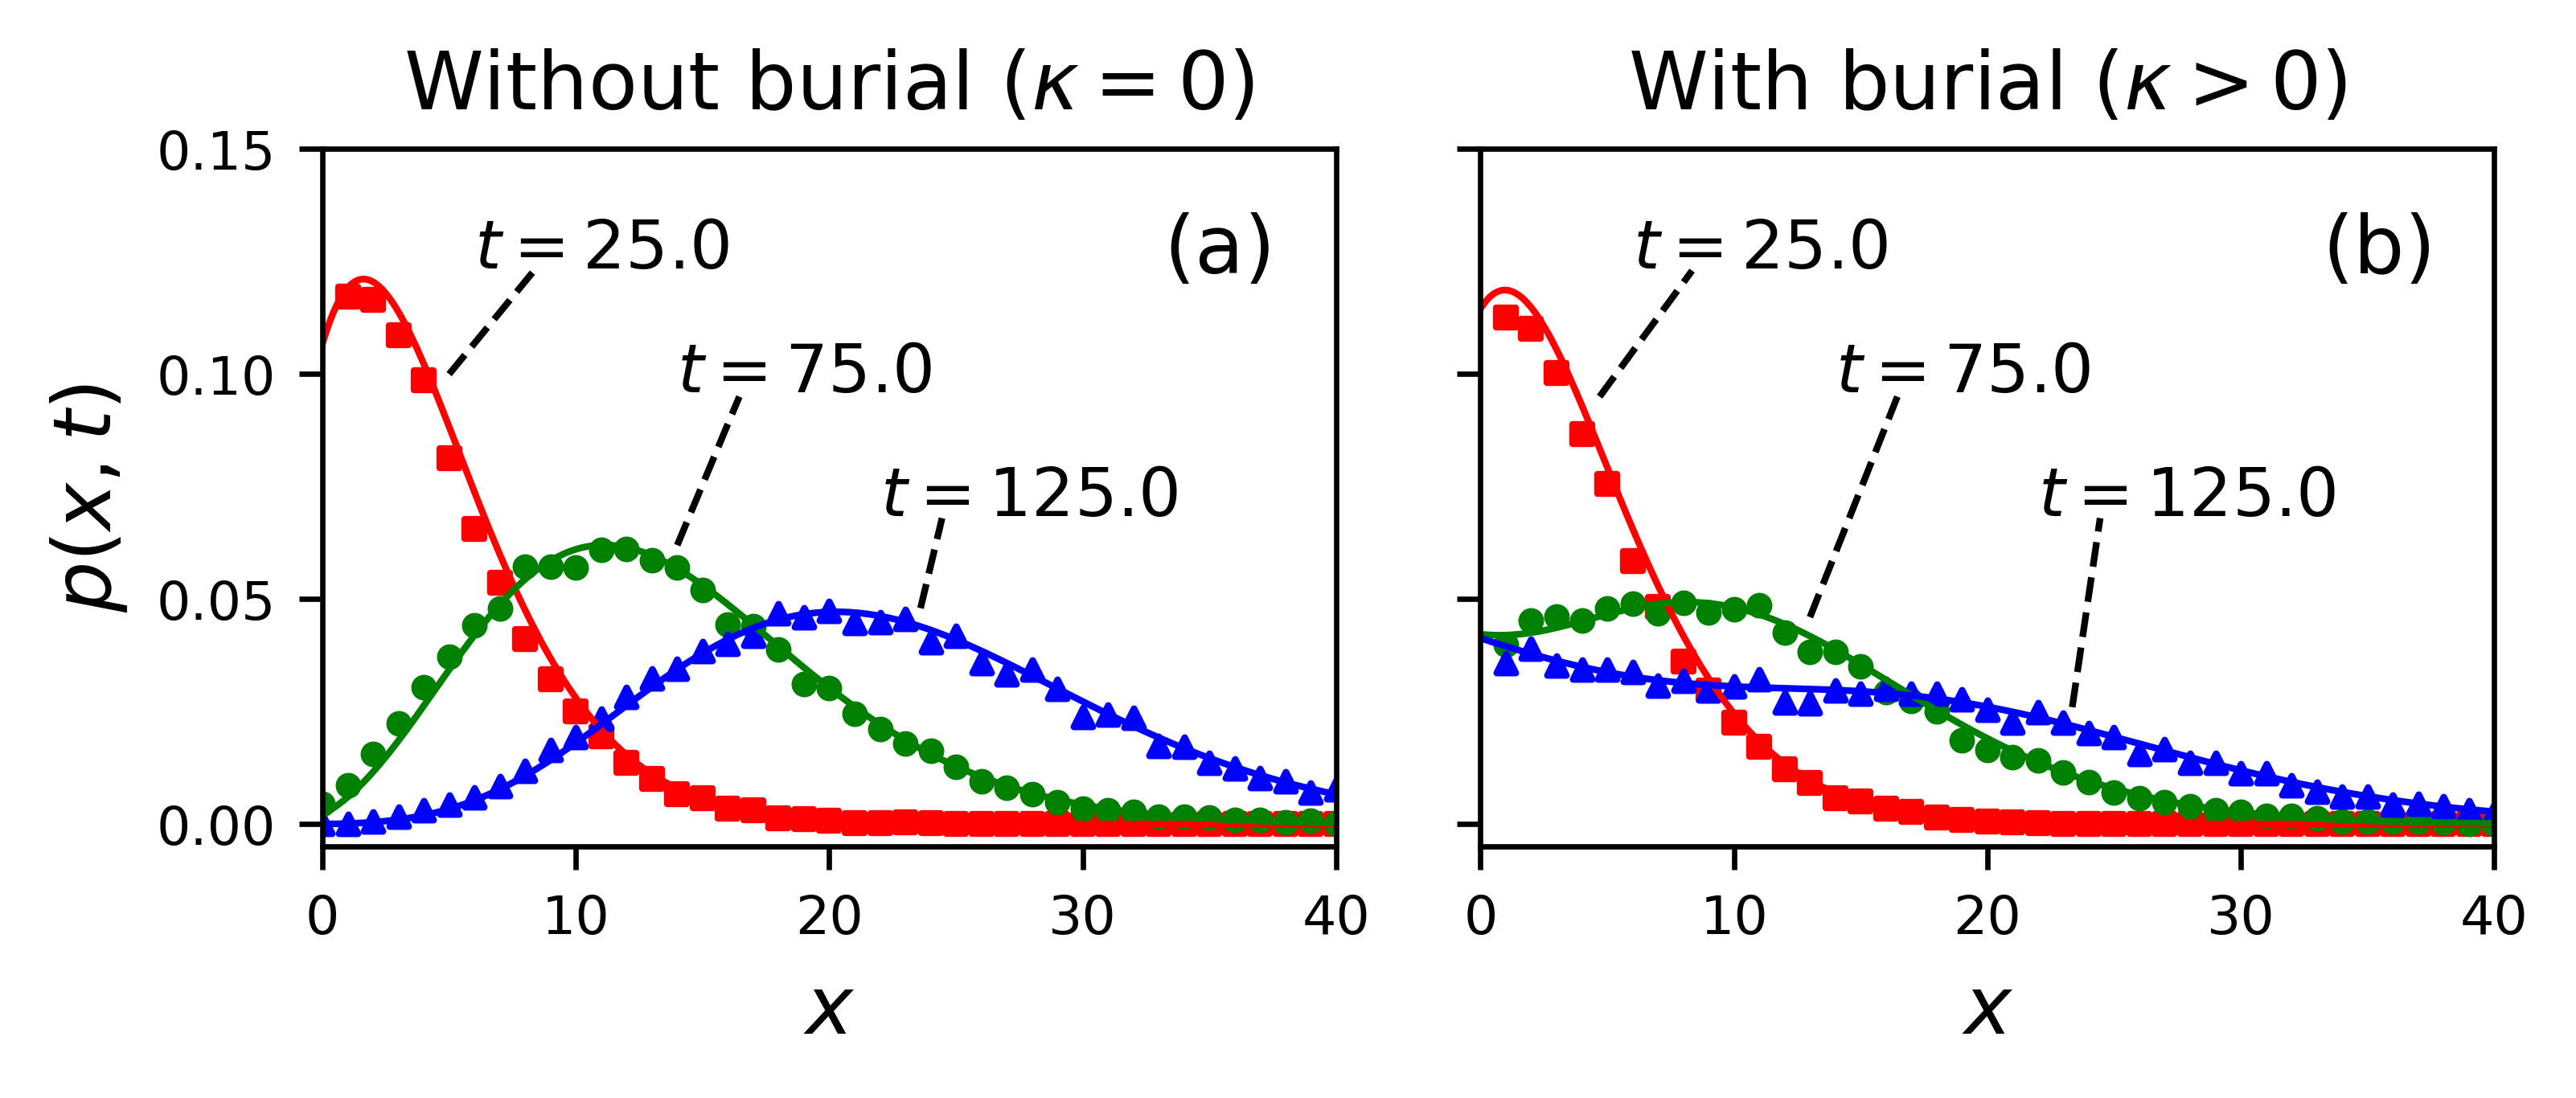
\includegraphics[width=\linewidth,keepaspectratio]{./figures/pdf-plot.png}
	\caption{Joint distributions for a grain to be at position $x$ at time $t$ are displayed for the choice $k_1=0.1$, $k_2=1.0$, $v=2.0$. Grains are considered initially at rest ($\theta_1=1$, $\theta_2=0$). The solid lines are the analytical distribution in equation (\ref{eq:pdf}), while the points are simulation results to show mathematical correctness. Colors pertain to different times. Units are unspecified, since our aim is to demonstrate the general characteristics of $p(x,t)$. Panel (a) shows the case $\kappa=0$ -- the absence of burial.
	In this case, the joint distribution tends toward Gaussian at large times \citep[e.g.][]{Einstein1937,Lisle1998}. Panel (b) shows the case when grains have rate $\kappa = 0.01$ to become buried while resting.
	Because of burial, the joint distribution tends toward a more uniform distribution than Gaussian. This shows a redistribution of probability to smaller values of $x$ due to the burial process \citep[cf.][]{Wu2019}. The redistribution is encoded mathematically by the Marcum Q-function terms in equation  (\ref{eq:pdf}). A similar tendency is seen in field studies of tracer dispersion in gravel bed rivers \citep[e.g.][]{Hassan1994}.}
	\label{fig:pdfs}
\end{figure}

% solution for theta_1=1: moments
 The first two moments and the positional variance are derived in appendix \ref{sec:appendixB}.
The moments are
\begin{align}
\bra x(t) \ket &= A_1 e^{(b-a)t}+B_1e^{-(a+b)t}+C_1, \label{eq:mean}\\
\bra x^2(t) \ket &= A_2(t)e^{(b-a)t}+B_2(t)e^{-(a+b)t}+C_2. \label{eq:second}
\end{align}
In these equations, $a = (\kappa + k_1+k_2)/2$ and $b = \sqrt{a^2-\kappa k_2}$ are effective rates having dimensions of inverse time.
The $A_i$, $B_i$, and $C_i$ are polynomials available in table \ref{table:params}.
The variance is
\be \sigma_x^2(t) = A(t)e^{(b-a)t} + B(t)e^{-(a+b)t} + C(t). \label{eq:var}\ee
$A, B,$ and $C$ are transcendental functions available in table \ref{table:params}.
This equation represents the scale-dependence of bedload diffusion for sediment gradually undergoing burial.
\begin{table}[!h]
	\centering
	\caption{Polynomials and transcendental functions used in the expressions of the mean (\ref{eq:mean}), second moment (\ref{eq:second}) and variance (\ref{eq:var}) of bedload tracers.}
	\label{table:params}
	\begin{tabular}{c}
		\toprule
		$\begin{aligned}[t]
		&A_1 = \frac{v}{2b}\big[\theta_2+\frac{k_1+\theta_2\kappa}{b-a}\big] \\
		&B_1 = -\frac{v}{2b}\big[\theta_2-\frac{k_1+\theta_2 \kappa}{a+b}\big] \\
		&C_1 =  -\frac{v}{2b}\big[\frac{k_1+\theta_2 \kappa}{b-a}+\frac{k_1+\theta_2 \kappa}{a+b}\big]\\
		&A_2(t) = \frac{v^2}{2b^3}\Big[(bt-1)[k_1+\theta_2(2\kappa + k_1 + b-a)]+\theta_2b \\
		&\hspace{3cm} + \frac{(\kappa+k_1)(\theta_2\kappa+k_1)}{(b-a)^2}[(bt-1)(b-a)-b]\Big]\\
		&B_2(t) = \frac{v^2}{2b^3}\Big[(bt+1)[k_1 + \theta_2(2\kappa+k_1-a-b)]+\theta_2b\\
		&\hspace{3cm} -\frac{(\kappa+k_1)(\theta_2\kappa+k_1)}{(a+b)^2}[(bt+1)(a+b)+b]\Big]\\
		&C_2 = \frac{v^2}{2b^3}(\kappa+k_1)(\theta_2 \kappa + k_1)\Big[\frac{2b-a}{(b-a)^2}+\frac{a+2b}{(a+b)^2}\Big]\\
		&A(t) = A_2(t)-2A_1C_1 - A_1^2\exp[(b-a)t]\\
		&B(t) = B_2(t)-2B_1C_1 - B_1^2\exp[-(a+b)t]\\
		&C(t) = C_2-C_1^2-2A_1B_1\exp[-2at]\\			
		\end{aligned}$\\
		\bottomrule
	\end{tabular}
\end{table}

The positional variance is plotted in figure \ref{fig:var} for conditions $\theta_1=1$ and $k_2\gg k_1 \gg \kappa$.
These conditions mean that all grains are initially at rest \citep[cf.][]{Wu2019}, motion intervals are typically much shorter than rests \citep[cf.][]{Einstein1937}, and sediment burial requires a much longer time than typical rests.
We concentrate on these conditions in this paper as they are most relevant to bedload diffusion in gravel-bed rivers, where sediment transport is typically rarefied and intermittent, and the burial process is relatively slow compared to surface resting times \citep[e.g.][]{Ferguson2002,Hassan1994}.
Figure \ref{fig:var} demonstrates that under these conditions the variance (\ref{eq:var}) shows three ranges of bedload diffusion with approximate power law scaling ($\sigma_x^2 \propto t^\gamma$), followed by a fourth range with no diffusion ($\sigma_x^2 = \text{const}$). We associate the first three ranges with the local, intermediate, and global ranges proposed by \citet{Nikora2001a,Nikora2002}, and identify the fourth range as resulting from the burial of all sediment grains.
We suggest to call the fourth range the geomorphic range, since any further transport in this range can occur only if scouring the bed exposes buried grains to the flow \citep[cf.][]{Nakagawa1980,Voepel2013,Martin2014}.
Using this terminology, we summarize that when $k_2\gg k_1 \gg \kappa$ and $\theta_1=1$, the variance in equation (\ref{eq:var}) expresses four scaling ranges of bedload diffusion: local, intermediate, global, and geomorphic.
However, we highlight that our model's representation of the geomorphic range is unrealistic due to our simplifying assumption of permanent burial \citep[cf.][]{Wu2019}. Properly modeling the geomorphic range will require investigations going beyond the one developed here.

\section{Discussion of scale-dependent bedload diffusion}
\label{sec:discussion}
\begin{figure}[t]	
	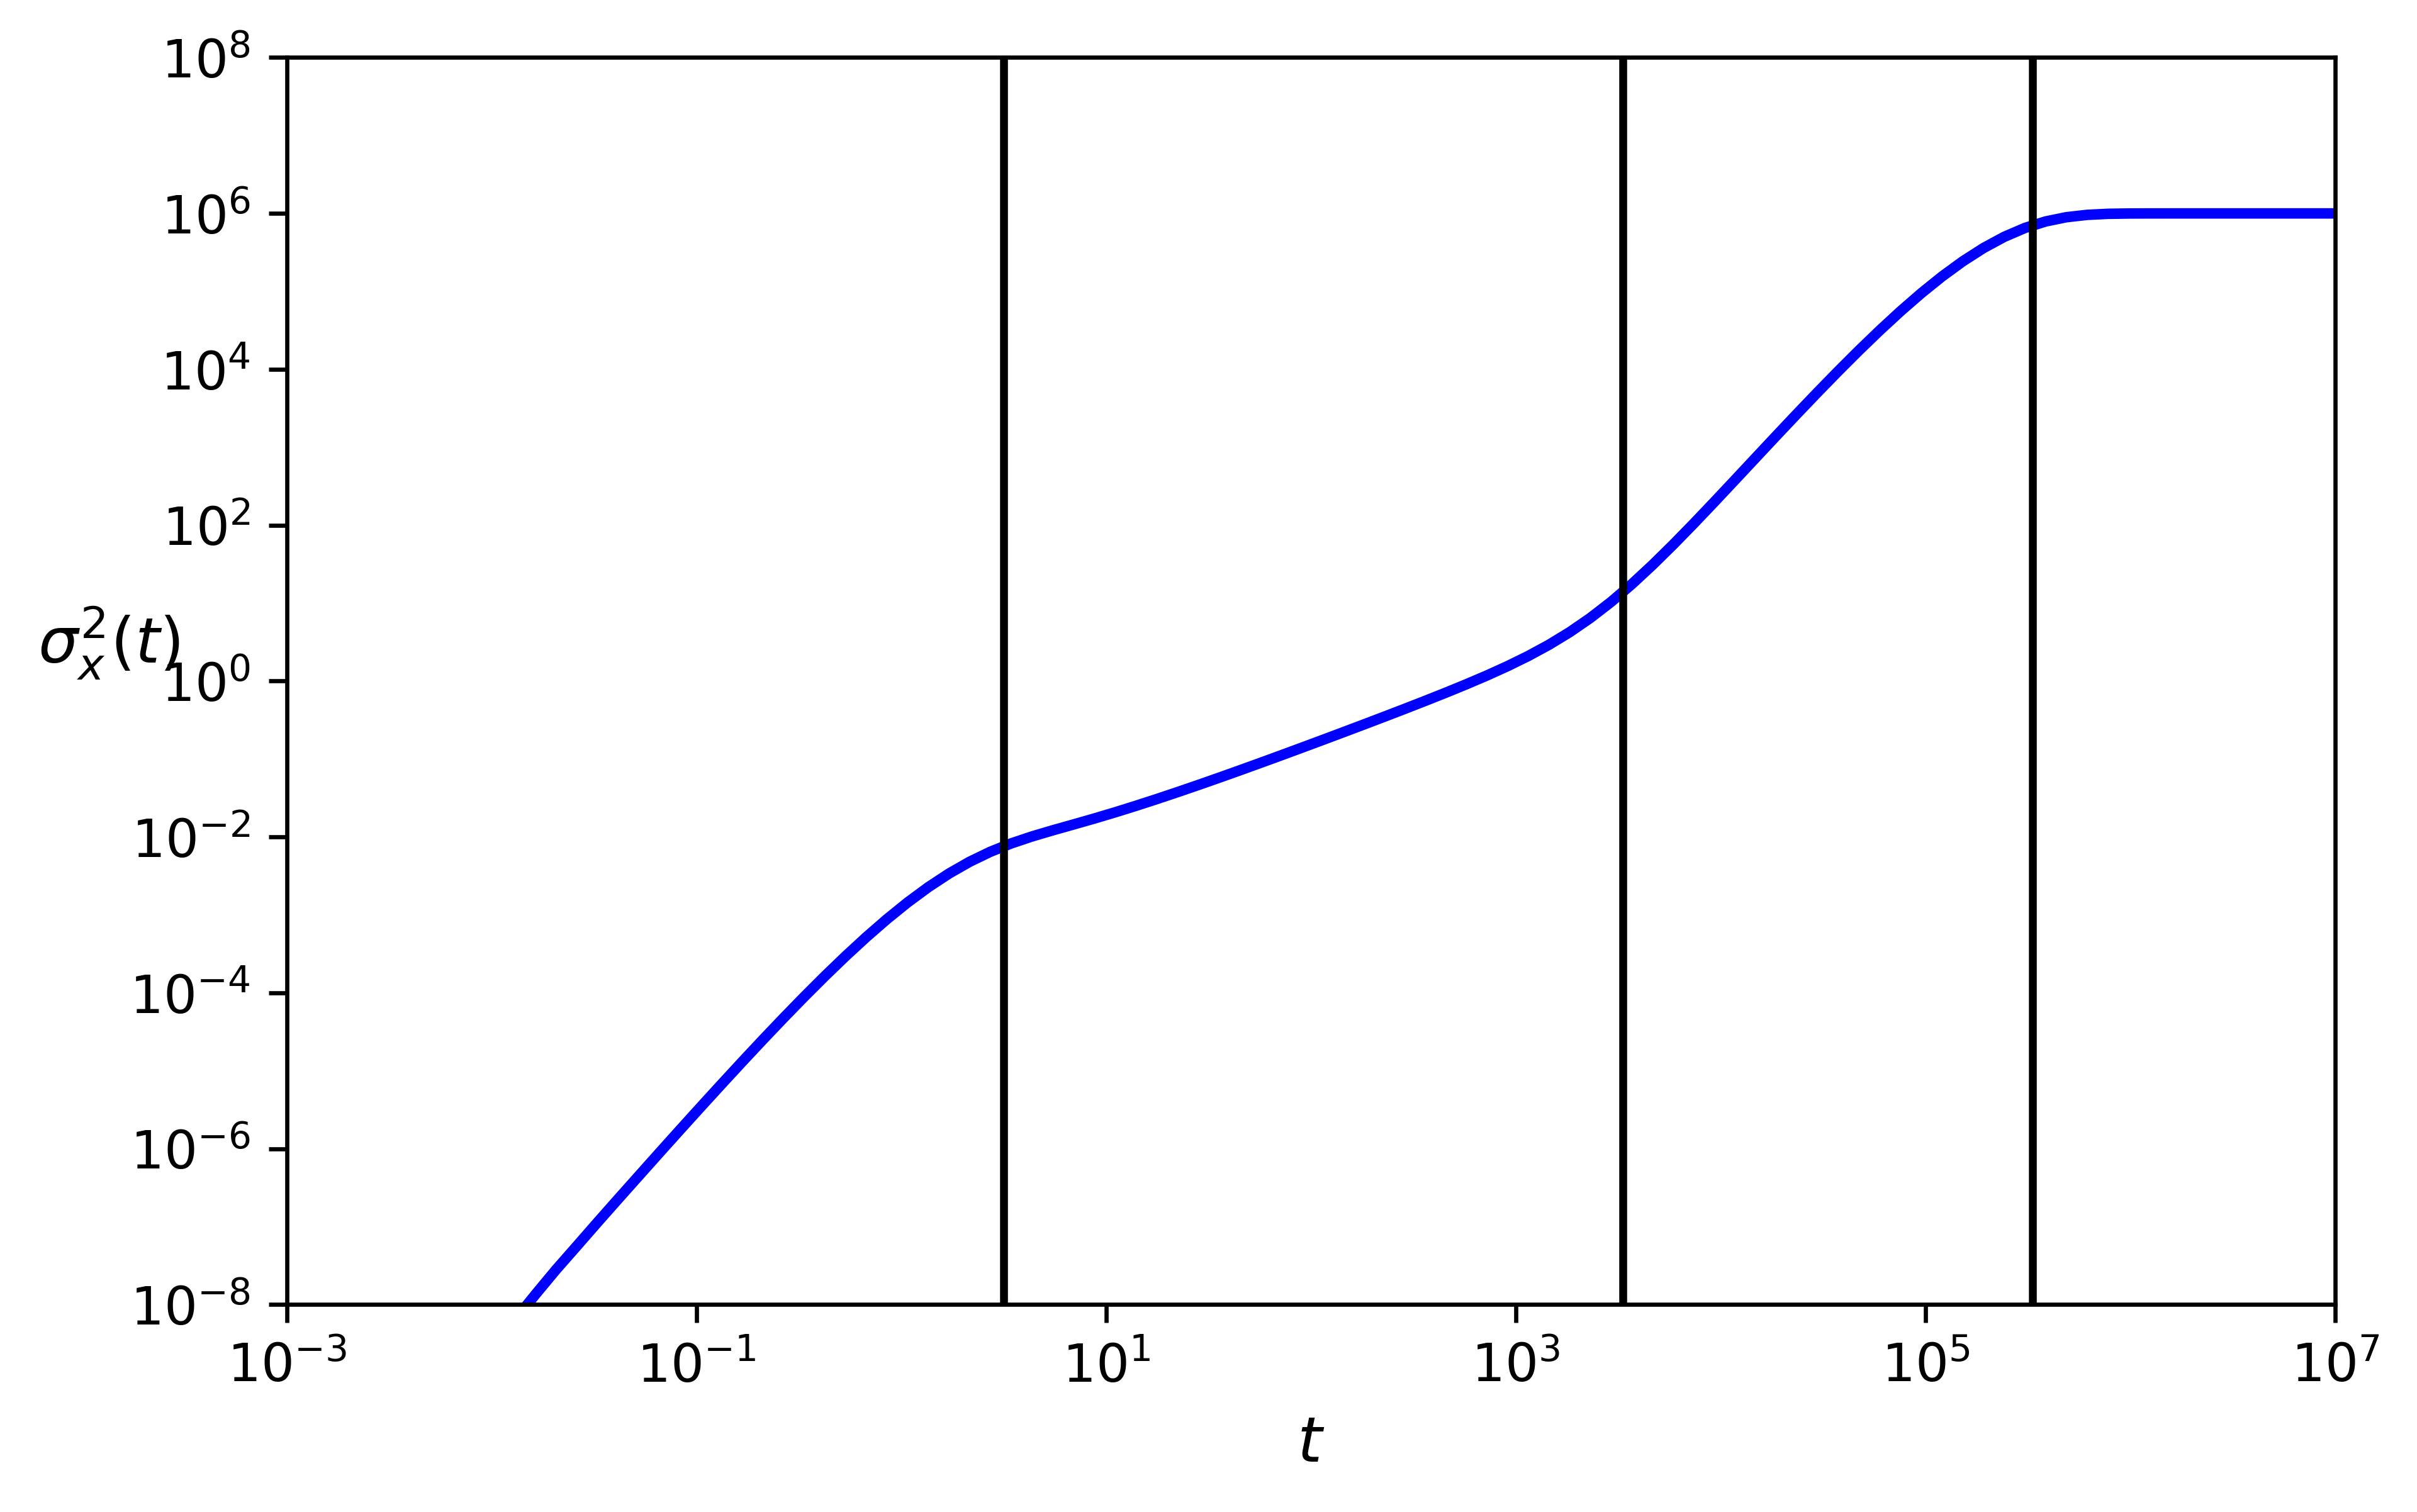
\includegraphics[width=\linewidth,keepaspectratio]{./figures/diffusion.png}
	\caption{The variance equation (\ref{eq:var}) is plotted for the parameters $1/k_2 = 1.5$s, $1/k_1 = 30.0$s, and $v=0.1$m/s. These values are comparable to laboratory flume experiments transporting small ($\sim 5$mm) gravels \citep[cf.][]{Lajeunesse2010,Martin2012}. The timescale of burial is set to $1/\kappa = 7200.0$s (two hours), and the initial condition is rest ($\theta_1=1$). The solid line is equation (\ref{eq:var}) while the points are directly simulated. When $k_2\gg k_1 \gg \kappa$, as as is the case in this plot, there are four distinct scaling ranges of $\sigma_x^2$: local, intermediate, global, and geomorphic. Within each range, a slope key is added to demonstrate the scaling $\sigma_x^2 \propto t^\gamma$. There are three crossovers between these ranges, denoted on the figure by vertical lines. Crossover times $T_L$, $T_I$, and $T_G$ are indicated at the bottom of the plot. They are given in equations (\ref{eq:TL}-\ref{eq:TG}) in terms of model parameters. }
	\label{fig:var}
\end{figure}

The model we have presented involves four parameters. These are the characteristic velocity $v$ of moving sediment and three key timescales: $1/k_2$, $1/k_1$, and $1/\kappa$.
These timescales represent the mean duration of motion, the mean duration of rest, and the mean duration of rest before burial occurs.
As shown in figure \ref{fig:var}, scaling laws $\sigma_x^2 \propto t^\gamma$ approximately characterize the diffusion in each scaling range.
The exponents $\gamma$ in each range result from competition between different terms in equation (\ref{eq:var}).
Between these ranges, there are crossover regions where the scaling is not a power law.
Because these crossover regions are relatively narrow, we can approximately characterize them with crossover times $T_L$, $T_I$, and $T_G$.
These times partition the diffusion ranges into $0< t < T_L$ (local), $T_L < t < T_I$ (intermediate), $T_I < t < T_G$ (global), and $T_G < t$ (geomorphic). 
Figure \ref{fig:var} depicts them as vertical lines.
To understand the bedload diffusion scale dependence expressed by equation \ref{eq:var}, we need to determine the exponents $\gamma$ of each range and relate the crossover times $T_L$, $T_I$, and $T_G$ between diffusion ranges to the model parameters $v$, $k_1$, $k_2$, and $\kappa$.

% now we figure out what the exponents are 
The diffusion exponents $\gamma$ in the local, intermediate, and global ranges can be extracted from two limiting cases of equation (\ref{eq:var}): (1) $t\ll 1/\kappa$, and (2) $1/k_2 \rightarrow 0$ while $vk_2 = \text{const}$.
Limit (1) corresponds to times so short a negligible amount of sediment burial has occurred, while limit (2) corresponds to times so long a motion interval appears as an instantaneous step having mean step length $l=vk_2$.
We evaluate these limits in appendix \ref{sec:appendixC} and obtain the diffusion exponents.
Local range diffusion has exponent $2 \leq \gamma \leq 3$ depending on the initial conditions $\theta_1$ and $\theta_2$.
When the initial conditions are pure, meaning one of the $\theta_i$ is zero, the local exponent is $\gamma=3$.
When grains start in a mixture of motion and rest states, meaning neither $\theta_i$ is zero, the local exponent is $\gamma=2$.
Intermediate range diffusion is simpler, and always has exponent $\gamma=1$, agreeing with the classic flume experiments based on visually tracing painted stones \citep[e.g.][]{Einstein1937,Yano1969a,Nakagawa1976}.
Finally, global range diffusion has exponent $1 \leq \gamma \leq 3$, depending on the ratio $k_1/\kappa$.
In the extreme case $k_1/\kappa \approx 0 $, $\sigma_x^2 \propto t$. 
However, in the opposite extreme $k_1/\kappa \rightarrow \infty$, $\sigma_x^2 \propto t^3$.
For general values of the ratio $\kappa/k_1$, the global exponent is a mixture of these extremes: $1 \leq \gamma \leq 3$. 
To summarize, when the model parameters satisfy $k_2\gg k_1 \gg \kappa$, so all three diffusion ranges exist, the variance (\ref{eq:var}) supports local range superdiffusion with exponent depending on the $\theta_i$, intermediate range normal diffusion, and global range superdiffusion with exponent depending on the ratio $k_1/\kappa$.
Finally, there is a geomorphic range of no diffusion ($\gamma=0$) associated with the eventual and permanent trapping of all sediment grains.

The crossover times between local, intermediate, global, and geomorphic ranges depicted in figure \ref{fig:var} are defined by
\begin{alignat}{2}
&T_L &&= \sqrt{\frac{1}{k_1}\frac{1}{k_2}}, \label{eq:TL}\\
&T_I &&= \sqrt{\frac{1}{k_1}\frac{1}{\kappa}},\label{eq:TI}\\
&T_G &&= \sqrt{\frac{1}{\kappa}\frac{k_1+k_2}{\kappa k_1}} \label{eq:TG}.
\end{alignat}
Each of these is a geometric mixture of two fundamental timescales of the model.
The crossover $T_L$ between local and intermediate ranges is a mixture of the mean times of a single rest and a single motion, while the crossover $T_I$ between intermediate and global ranges is a mixture of the mean time of a single rest and the mean time required for a resting grain to become buried.
The crossover $T_G$ between global and geomorphic ranges is more difficult to understand. We came to equation (\ref{eq:TG}) by reasoning that the first grains to trap will be those which have almost always been at rest since $t=0$. 
These will trap at $t\sim1/\kappa$, which is the first timescale in equation (\ref{eq:TG}). The last grains to trap will be those which are likely to be in motion at relatively large times, since this means they have not been in the resting state in which they are susceptible to burial.
By analogy to the two-state mobile-immobile model of \citet{Ancey2006}, we reason that if grains have been in transport a relatively long time and has not been buried, the fraction of time they spend in motion will be $(1/k_2)/(1/k_1+1/k_2) = k_1/(k_1+k_2)$. For these grains, the trapping rate is effectively reduced to $\kappa k_1/(k_1+k_2)$, which is the second timescale in equation (\ref{eq:TG}).
We have visually tested the crossover time expressions (\ref{eq:TL}-\ref{eq:TG}) for many parameter choices. As long as they satisfy $k_2\gg k_1 \gg \kappa$, these expressions provide an adequate characterization of the crossover locations between diffusion regimes.
Equations (\ref{eq:TL}) and (\ref{eq:TI}) are especially trustworthy.
However, by contriving large values of $k_2$, it is possible to drive $T_G$ to ever larger values, in effect making the crossover region between global and geomorphic ranges arbitrarily wide.
Ultimately, we suggest these expressions be used with care and in consideration of the idealization being made in representing a crossover region of finite width by a single characteristic time. We suggest the width and characteristics of the crossover regions between the power-law ranges of bedload transport as an open research problem in need of clarification.

We have extended earlier bedload diffusion models to describe four ranges of diffusion instead of one or two.
Earlier models can be accessed through the two simplified limits used earlier to extract the scaling exponents $\gamma$.
As discussed in appendix \ref{sec:appendixC}, limit (1) leads directly to the model developed by \citet{Lisle1998} to describe soil transport within a sheet flow, while limit (2) implies identical diffusion characteristics as the active layer formulation of bedload transport gradually undergoing burial developed by \citet{Wu2019}.
Each of these subsequently limits to the original descriptions of \citet{Einstein1937} and his followers \citep[e.g.][]{Hubbell1964, Nakagawa1976, Yano1969,Shen1980}.
\citet{Lisle1998} generalized the Einstein model, which is an infinite velocity diffusion model involving instantaneous steps, to include a finite velocity and duration of motion.
Although \citet{Lisle1998} only mention this anecdotally, their generalization leads to two stages of diffusion, in constrast to the single range of \citet{Einstein1937} and followers \citep[e.g.][]{Yano1969, Nakagawa1976}.
One is local range superdiffusion and the other is an intermediate range normal diffusion.
This is shown in appendix \ref{sec:appendixC}.
\citet{Wu2019} developed an active layer formulation of fluvial bedload transport where sediment grains can be transferred from the active layer (surface) to a substrate layer (burial) with a constant probability per unit time.
They simplified the problem by considering permanent burial (as we have) and motion by instantaneous steps, deriving two stages of diffusion that we identify as an intermediate range normal diffusion and a global range superdiffusion.
Our model extends these two works and links them into the formalism of multi-state CTRWs \citep[e.g.][]{Weiss1994} that was implicitly applied by \citet{Einstein1937}. Further developments may benefit from staying close to these unifying ideas from the physics literature.

We identify two key implications of the model we've presented in this letter.
First, this work is the first to confine the range over which normal diffusion of bedload is expected. We can infer from the classic flume tracer studies that normal diffusion is expected of bedload when the timescale of observation is neither sufficiently small to resolve individual motions nor sufficiently large to resolve the trapping of tracers by sediment burial \citep{Einstein1937, Einstein1942, Yano1969, Yano1969a, Nakagawa1976}. 
We have quantified this observation. When the timescale under consideration satisfies $T_L<t<T_I$, with $T_L$ and $T_I$ given by equations (\ref{eq:TL}) and (\ref{eq:TI}), we expect normal bedload diffusion $\sigma_x^2 = D_dt$. This heuristic may be useful to discern when and if simple stochastic models of bedload transport may be relevant to environmental science considerations such as contaminant transport \citep[e.g][]{Malmon2005,Macklin2006} or aquatic habitat restoration \citep[e.g.][]{Gaeuman2017}.
Second, the model links bedload transport understanding across scales. In practice, we might measure sediment diffusion within a channel on one timescale with intent to apply our knowledge at longer or shorter timescales. Often, the measurement timescale is limited by practical reasons. For example, we could determine $k_1$ and $k_2$ by measuring the virtual velocity and diffusivity of sediment tracers in the intermediate range \citep[e.g.][]{Hassan2017}. With an estimate of the trapping rate $\kappa$, equation \ref{eq:var} can predict diffusion characteristics on the global range $T_I<t<T_G$, which is more difficult to study experimentally.


Finally, we highlight some limitations of our model and suggest some ideas for future research.
Perhaps the most obvious limitation is that we have considered burial to be a permanent condition, which led to no transport or diffusion in the geomorphic range of timescales.
In actuality, sediment burial is a temporary process relating to the scour and fill of the sedimentary bed \citep[e.g.][]{Hassan1994,Wong2007,Voepel2013,Martin2014}, and there is a need to better quantify the timescales of this process.
In particular, there have been no measurements so far of the sediment burial rate $\kappa$ (or $\chi$ in the notation of \citet{Wu2019}). In principle, this could be extracted from flume experiments by timing the duration that tracers can rest on the surface before they become buried.
Furthermore, existing theoretical studies have attributed sediment resting periods to any resting sediment, whether buried or not \citep[e.g.][]{Voepel2013,Martin2014}.
We argue this is a process-independent concept of sediment resting.
This concept implies heavy-tailed sediment resting time distributions \citep[e.g.][]{Martin2012,Hassan2013, Olinde2015}.
However, one can envision multiple trapping processes in coexistence within channels, such as sediment trapping by burial \citep[e.g.][]{Hassan1994,Haschenburger2013,Ferguson2002} and by stranding on top of bars \citep[e.g.][]{Ferguson2002,Bradley2017} and floodplains \citep[e.g.][]{Malmon2003}.
We suggest it may be useful to treat sediment resting intervals of sediment exposed on the surface differently than resting intervals of trapped sediment.
This opens up the possibility to include multiple trapping processes which may act simultaneously and on different timescales into fluvial sediment diffusion models.
A second limitation we have already alluded to: this limitation is shared by all stochastic bedload transport models we are aware of.
This is that the role of channel morphology and its evolution on statistical characteristics of sediment transport are experimentally well-known and appreciable \citep[e.g.][]{Pyrce2005,Kasprak2014, Hassan2017}, but this appears to us to have been essentially neglected in models.
There is a need to better understand the statistical characteristics of bedload transport in a context of channel morphology.
Presumably, this imparts spatial and temporal variations into these statistics, or it possibly renders them ill-defined, which would be an unfortunate state of affairs.
This interrelationship between morphology and transport deserves ever more attention.
The connections are apparently more intimate than some classical researchers realized, if the recent observations of stick-slip motions of bars are any indication \citep{Dhont2018}.
Finally, with regard to these limitations we highlight that the random walk formalism from the physics literature we have used in this letter \citep{Weiss1994} has been carefully extended to conditions where mobility characteristics vary across space and time. This is called a random walk in a random environment and is a popular concept in biological transport \citep[e.g.][]{Codling2008}. Perhaps there are lessons in this literature for river geophysics. Can the morphologically active river channel be treated as a random environment while bedload grains move in random walks?
More openness to interdisciplinary research might provide new traction on the problem of appropriately describing bedload transport from local to geomorphic scales.

\section{Conclusion}
\label{sec:conclusion}
We have developed a random walk model between alternating mobile and immobile states with a possibility of trapping from the immobile state, and we have used it to describe the diffusion of bedload sediment transporting through a river channel as it gradually becomes buried.
This ultimately extends the original diffusion model of \citet{Einstein1937}.
To our knowledge, this model is the first analytical description of bedload diffusion across local, intermediate, and global timescales.
Pushing the ideas of \citet{Nikora2002} somewhat further, we have suggested a geomorphic range of diffusion to describe the range at timescales larger than the global range that is not properly characterized by existing models of bedload diffusion that neglect morphodynamic processes.
Our model implies a possibility to use information from experiments conducted on one timescale to understand sediment diffusion phenomena and related problems such as channel morphology \citep[e.g.][]{Church2006, Hassan2017} and environmental issues \citep[e.g.][]{Macklin2006,Gaeuman2017} on other timescales.
The next step to incorporate the bed scour process which re-exposes buried sediment into a bedload diffusion model like the one we have presented here.
This will overcome the approximation of permanent burial and better resolve the diffusion characteristics of the geomorphic range. 
The multi-state random walk formalism we used here should readily accommodate this extension \citep[e.g.][]{Weiss1994} and others aiming to incorporating more physical processes into Einstein's modeling paradigm of fluvial sediment diffusion.


 




 


\appendix

\section{Calculation of the distribution function}
\label{sec:appendixA}
Double transforming (\ref{eq:x}-\ref{eq:y}) using the definition (\ref{eq:doubletransform}) gives

\begin{alignat}{2}
&\tom_{1T}(\eta,s) &&= \theta_1 \tg_1(\eta,s) + \tom_2(\eta,s)\tg_1(\eta,s)-\tom_{1F}(\eta,s),\\
&\tom_{1F}(\eta,s) &&= \theta_1\tg_1(\eta,s+\kappa) + \tom_2(\eta,s)\tg_1(\eta,s+\kappa),\\
&\tom_2(\eta,s) &&= \theta_2 \tg_2(\eta,s) + \tom_{1F}(\eta,s)\tg_2(\eta,s).
\end{alignat}
This purely algebraic system solves for 
\begin{alignat}{2}
&\tom_{1T}(\eta,s) &&= \frac{\theta_1 + \theta_2 \tg_2(\eta,s)}{1-\tg_1(\eta,s+\kappa)\tg_2(\eta,s)}\big\{\tg_1(\eta,s)-\tg_1(\eta,s+\kappa) \big\}, \label{eq:A} \\
&\tom_{1F}(\eta,s) &&= \frac{\theta_1 + \theta_2 \tg_2(\eta,s)}{1-\tg_1(\eta,s+\kappa)\tg_2(\eta,s)}\tg_1(\eta,s+\kappa),\\
&\tom_{2}(\eta,s) &&= \frac{\theta_2 + \theta_1 \tg_1(\eta,s+\kappa)}{1-\tg_1(\eta,s+\kappa)\tg_2(\eta,s)}\tg_2(\eta,s). 
\end{alignat}
Double transforming (\ref{eq:b}-\ref{eq:z}) gives
\begin{align}
\tp_0(\eta,s) &= \frac{1}{s}\tom_{1T}(\eta,s),\\
\tp_1(\eta,s) &= \theta_1 \tG_1(\eta,s) + \tom_2(\eta,s) \tG_1(\eta,s),\\
\tp_2(\eta,s) &= \theta_2 \tG_2(\eta,s) + \tom_{1F}(\eta,s)\tG_2(\eta,s).\label{eq:Z}
\end{align}
The total probability is $p(x,t) = p_0(x,t) + p_1(x,t) + p_2(x,t)$. Using equations (\ref{eq:A}-\ref{eq:Z}) this becomes, in the double Laplace representation, 
\begin{multline}
\tp(\eta,s) = \frac{1}{s}\frac{\theta_1 + \theta_2 \tg_2(\eta,s)}{1-\tg_1(\eta,s+\kappa)\tg_2(\eta,s)}\big\{\tg_1(\eta,s)-\tg_1(\eta,s+\kappa) \big\} \\
+\frac{\theta_1\big[\tG_1(\eta,s) + \tg_1(\eta,s+\kappa)\tG_2(\eta,s)\big]+ \theta_2\big[\tG_2(\eta,s) + \tg_2(\eta,s)\tG_1(\eta,s)\big]}{1-\tg_1(\eta,s+\kappa)\tg_2(\eta,s)}. \\
\label{eq:lap}
\end{multline}
Plugging the propagators outlined in equations (\ref{eq:prop1}-\ref{eq:prop2}) into equation (\ref{eq:lap}) gives 
\be \tilde{p}(\eta,s) = \frac{1}{s}\frac{(s+\kappa + k')s  + \theta_1(s+\kappa )\eta v+ \kappa k_2}{(s+\kappa+k_1)\eta v+(s+\kappa+k')s + \kappa k_2}.\label{eq:nicedist}\ee
In this equation, $k'=k_1+k_2$, and we have used the normalization requirement of the initial probabilities $\theta_1 + \theta_2 = 1.$
The double inverse transform of this equation provides the distribution $p(x,t)$.
It is convenient to invert the transform over $\eta$ first.
Using the results 15.103 (transform of exponential), 15.123 (transform of derivative), and 15.141 (transform of Dirac delta function) from \citet{Arfken1985} provides 
\begin{multline} \tp(x,s) = \theta_1 \frac{s+\kappa}{s(s+\kappa + k_1)}\delta(x) + \frac{1}{v} \Big(\frac{(s+\kappa+k')s+\kappa k_2}{s(s+\kappa+k_1)} \\- \frac{\theta_1(s+\kappa)[s(s+\kappa+k_1)+\kappa k_2]}{s(s+\kappa+k_1)^2}\Big)
\exp\Big[-\frac{(s+\kappa+k')s+\kappa k_2}{s+\kappa+k_1}\frac{x}{v}\Big].\end{multline}
Taking the remaining inverse transform over $s$, applying results 15.152 (substitution), 15.164 (translation), and 15.175 (transform of $te^{kt}$) from \citet{Arfken1985}, and defining the shorthand notations $\tau = k_1(t-x/v)$, $\xi = k_2 x/v$, and $\Omega = (\kappa + k_1)/k_1$, gives the simpler form 
\begin{multline}
p(x,t) = \theta_1\Big[1-\frac{k_1}{\kappa + k_1}\big(1-e^{-(\kappa + k_1)t}\big)\Big]\delta(x) + \frac{1}{v}\exp[\Omega \tau - \xi]\\
\times \El^{-1}\Big\{\Big( \theta_2 + \frac{\theta_1k_1+\theta_2 k_2}{s}+\frac{\theta_1k_1k_2}{s^2} + \frac{\theta_2\kappa k_2}{s(s-\kappa-k_1)} + \frac{\theta_1\kappa k_1 k_2}{s^2(s-\kappa-k_1)}\Big)\\
\times\exp\big[\frac{k_1 \xi}{s}\big];\tau/k_1\Big\}.
\end{multline}
Using entries 2.2.2.1, 2.2.2.8, and 1.1.1.13 from \citet{Prudnikov1992a} in conjunction with the definition of the Marcum Q-function $ \mathcal{P}_\mu(x,t)$ \citep[e.g.][]{Temme1996}, and inserting the Heaviside functions to account for the fact that grains can neither travel backwards nor at speeds exceeding $v$, we finally arrive at equation \ref{eq:pdf} for the joint distribution $p(x,t)$.

\section{Calculation of the moments}
\label{sec:appendixB}
We leverage equation \ref{eq:momenttrick} to compute the first two moments of position $x$ and ultimately its variance. The first two derivatives of the double Laplace transformed distribution (\ref{eq:nicedist}) are
\be \partial_\eta \tp(\eta,s) = -v \frac{1}{s}\frac{[(s+\kappa + k')s + \kappa k_2][\theta_2(s+\kappa) + k_1]}{[\eta v(s+\kappa +k_1) + (s+ \kappa + k')s+\kappa k_2]^2},\ee
\be \partial_\eta^2 \tp(\eta,s) = 2v^2 \frac{1}{s} \frac{(s+\kappa+k_1)[(s+\kappa + k')s+\kappa k_2][\theta_2(s+\kappa) + k_1]}{[\eta v(s+\kappa + k_1) + (s+\kappa + k')s+ \kappa k_2]^3}.\ee
Evaluating these at $\eta=0$ and applying equation (\ref{eq:momenttrick}) provides the Laplace transformed moments
\be  \frac{\bra\tilde{x}(s)\ket} {v} = \frac{1}{s}\frac{\theta_2(s+\kappa)+k_1}{(s+\kappa+k')s+\kappa k_2} = \frac{1}{s} \frac{\theta_2(s+\kappa)+k_1}{(s+a+b)(s+a-b)}\label{eq:lapmean},\ee
\be \frac{\bra \tilde{x}^2(s) \ket}{2v^2} = \frac{1}{s} \frac{(s+\kappa+k_1)(\theta_2(s+\kappa)+k_1)}{[(s+\kappa+k')s+\kappa k_2]^2}=  \frac{1}{s}\frac{(s+\kappa+k_1)(\theta_2(s+\kappa)+k_1)}{(s+a+b)^2(s+a-b)^2}.\label{eq:lapsecondmom}\ee
The parameters $a= (\kappa+k')/2$ and $b^2 = a^2 -\kappa k_2$ were introduced to factorize the denominators.
These equations can be inverted using the properties 15.164 (translation), 15.11.1 (integration), and 15.123 (differentiation) from  \citet{Arfken1985} after expansion in partial fractions.
For the mean, the calculation is
\begin{align}
\frac{2b}{v}\bra x \ket &= \big[\theta_2 + (k_1+\theta_2 \kappa)\int_0^t dt\big]\El^{-1}\Big\{ \frac{1}{s+a-b}-\frac{1}{s+a+b};t\Big\}\\
&= \Big[\theta_2 + \frac{k_1+\theta_2\kappa}{b-a}\Big]e^{(b-a)t} - \Big[\theta_2 - \frac{k_1+\theta_2\kappa}{a+b}\Big]e^{-(a+b)t} - \Big[\frac{k_1+\theta_2\kappa}{b-a} + \frac{k_1+\theta_2\kappa}{a+b}\Big].
\end{align}
This equation rearranges to (\ref{eq:mean}).
The second moment (\ref{eq:lapsecondmom}) is 
\begin{multline}
\frac{2b^2}{v^2}\bra x^2 \ket = \Big[\theta_2(\delta(t) + \partial_t) + (\theta_2(2\kappa + k_1)+k_1) + (\kappa+k_1)(\theta_2\kappa+k_1)\int_0^t dt \Big] \\
\times \El^{-1}\Big\{ \frac{1}{(s+a-b)^2} + \frac{1}{(s+a+b)^2}-\frac{1}{b(s+a-b)}+\frac{1}{b(s+a+b)};t\Big\}.
\end{multline}
This becomes 
\begin{multline}
\frac{2b^3}{v^2}\bra x^2 \ket = \Big[\theta_2\partial_t + [\theta_2(2\kappa+k_1)+k_1] + (\kappa+k_1)(\theta_2\kappa+k_1)\int_0^tdt\Big]\\
\times \Big((bt-1)e^{(b-a)t}+(bt+1)e^{-(a+b)t}\Big),
\end{multline}
which evaluates to equation (\ref{eq:second}).
$\sigma_x^2 = \bra x^2 \ket - \bra x \ket^2$ derives the variance in equation (\ref{eq:var}).

\section{Limiting behavior of the moments}
\label{sec:appendixC}
The easiest approach to extract the earlier results of \cite{Wu2019}, \citet{Lisle1998}, and \citet{Einstein1937} for the moments and positional variance as limiting cases is to use the Laplace transformed moments (\ref{eq:lapmean}) and (\ref{eq:lapsecondmom}) as a starting point.
An alternate approach is to take limits in the moments (\ref{eq:mean}) and (\ref{eq:second}) directly, but this is more challenging.
First we obtain the \citet{Wu2019} model as a limit case. 
These authors accounted for sediment burial considering motions to be instantaneous.
They characterized sediment movement by a thin-tailed step length distribution, implicitly involving an infinite motion velocity.
To obtain their conclusions on bedload diffusion, we send the mean duration of motion to zero ($1/k_2\rightarrow 0$), the velocity to infinity ($v\rightarrow \infty$), and we hold the mean step distance $l = v/k_2$ constant.
We use the initial condition that grains start at rest ($\theta_1=1$).
Enacting these limits in equations (\ref{eq:lapmean}) and (\ref{eq:lapsecondmom}) provides
\begin{align}
\bra \tilde{x} \ket &= k_1l\frac{1}{s(s+\kappa)},\\
\bra \tilde{x}^2 \ket &= 2l^2k_1 \frac{s+\kappa+k_1}{s(s+\kappa)^2}.
\end{align}
Inverting these equations and introducing the variables $c=lk_1$ (an effective velocity) and $D_d = l^2k_1$ (a diffusivity) provides positional variance
\be \sigma_x^2(t) = \frac{2D_d(1-e^{-\kappa t})}{\kappa} + \frac{(1-e^{-2\kappa t}-2e^{-\kappa t}\kappa t)c^2}{\kappa^2}.\ee
This is mathematically identical to the key result of \citet{Wu2019}, providing two ranges of diffusion when $\kappa \ll k_1$. One is normal and the other, induced by sediment burial, is superdiffusive.
From here, the \citet{Einstein1937} result can be obtained by turning off the burial process ($\kappa \rightarrow 0$):
\be \sigma_x^2(t) = 2D_d t.\ee
This represents a single range of normal diffusion \citep[cf.][]{Hubbell1964,Nakagawa1976}.

The \citet{Lisle1998} result can be obtained similarly. For this case, we neglect the burial process $(\kappa \rightarrow 0$) but retain the finite velocity and motion duration in equations (\ref{eq:lapmean}) and (\ref{eq:lapsecondmom}).
For the initial condition $\theta_1=1$, this provides 
\begin{align}
\bra \tilde{x} \ket &= vk_1 \frac{1 }{s^2(s+k')}, \label{eq:li1}\\
\bra \tilde{x}^2 \ket &= 2v^2k_1 \frac{s+k_1}{s^3(s+k')^2}. \label{eq:li2}
\end{align}
Inverting these equations provides the variance when $t\ll 1/\kappa$:
\be \sigma_x^2 = 2v^2\frac{k_1}{k'^4}\Big(k_1\big[\frac{1}{2} - k'te^{-k't} - \frac{1}{2} e^{-2k't}\big] + k_2\big[-2+k't + (2+k't)e^{-k't}\big]\Big).\ee
This result encodes two stages of diffusion: at small times there is superdiffusion $\sigma_x^2 \propto t^\gamma$ with $\gamma = 2-3$ depending on the initial condition, and at longer times there is normal diffusion. This links back to the Einstein model in the limit of instantaneous steps: $1/k_2 \rightarrow 0$ and $v\rightarrow \infty$ while $v/k_2 = l$.

Finally, we examine the limit $t\rightarrow 0 $ while leaving $\kappa \neq 0$. This will highlight the effect of initial conditions on the local range superdiffusion.
By applying Tauberian theorems, we can argue the $ t \rightarrow 0$ variance is determined by the $s\rightarrow \infty$ limits of (\ref{eq:lapmean}) and (\ref{eq:lapsecondmom}) \citep[e.g.][]{Weiss1994, Weeks1998}.  Expanding these equations in powers of $1/s \ll 1$ and inverting the resulting transforms gives
\begin{align} \bra x \ket &= v \theta_2 t + \frac{1}{2}v(\theta_1k_1-\theta_2k_2)t^2 + O(t^3),\\
\bra x^2 \ket &= v^2\theta_2 t^2 + \frac{1}{3}v^2(\theta_1k_1-2\theta_2k_2)t^3+ O(t^4).
\end{align}
Taking only leading order terms for each option of $\theta_1$ and $\theta_2$, these equations provide the asymptotic ($t\rightarrow 0$) variance 
\be \sigma_x^2(t) \sim v^2\theta_1\theta_2t^2 + \frac{1}{3}v^2(\theta_1k_1+\theta_2k_2)t^3.\ee
This equation shows the effect of initial conditions on the diffusion characteristics of the local range.

\acknowledgments
J. Pierce acknowledges helpful exchanges with Eduardo Daly and Peter H{\"a}nggi during the early stages of this work. He would like to thank Melinda Saunders and Leonardo Golubovic for their careful guidance in mathematics through the years. M. Hassan is supported by an NSERC Discovery grant. The Python simulation code is available at \sloppy
\url{https://github.com/kevinkayaks/rw-diffu}.

\bibliography{biblio.bib}
\end{document}